\documentclass[12pt]{article}


\usepackage{tabularx}
\usepackage[table]{xcolor}
\usepackage{multirow}

\usepackage{graphics}
\usepackage{graphicx}

\usepackage{amsmath, amssymb}
\usepackage{mathtools}

\usepackage[margin=1.1in,footskip=.25in]{geometry}

\usepackage[most]{tcolorbox}

\tcbset{
    frame code={}
    center title,
    left=10pt,
    right=10pt,
    top=10pt,
    bottom=10pt,
    colback=gray!5,
    colframe=gray,
    width=\dimexpr\textwidth\relax,
    enlarge left by=0mm,
    boxsep=5pt,
    arc=0pt,outer arc=0pt,
}


\usepackage{xepersian}
\settextfont[Scale=1]{Vazir}

\renewcommand{\baselinestretch}{1.3} 



\begin{document}



\noindent
هوش مصنوعی
\lr{(Artificial intelligence)}
 چیست ؟

\vspace{10pt}


\begin{tcolorbox}
به توانایی فکر کردن و یادگرفتن یک برنامه ی کامپیوتری یا ماشین  هوش مصنوعی می گویند 
\end{tcolorbox}

\vspace{30pt}

\noindent
عامل
\lr{(Agent)}
 چیست ؟ ساختار عامل واکنشی ساده را رسم کنید ؟

\vspace{10pt}

\begin{tcolorbox}
هر عاملی با محیط اطراف خود در ارتباط است و این عامل محیط  اطراف خود را از طریق حسگر ها درک کند و از طریق عملگرها در آن محیط اقدام کند و تاثیر می گذارد .
\end{tcolorbox}


\begin{tcolorbox}
عامل های واکنشی ساده دارای جدول جستجوی آسان هستند و تعداد وضعیت ها در آنها می توانند توسط قانون شرط-عملکرد خلاصه شوند 
\end{tcolorbox}

\begin{center}
	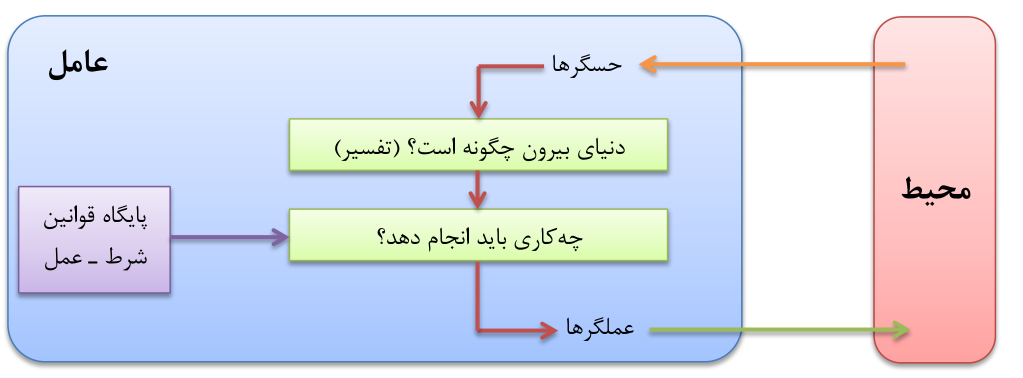
\includegraphics[scale=0.6]{./Untitled.png}
\end{center}

\begin{center}
	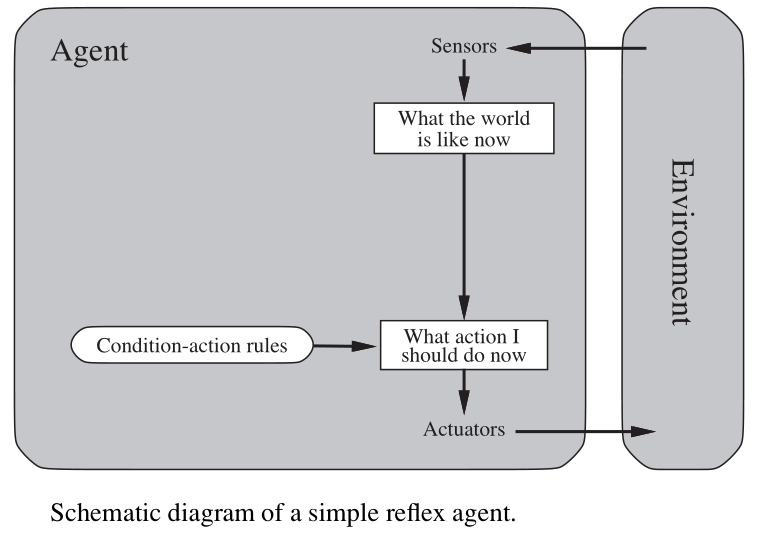
\includegraphics[scale=0.6]{./simple_reflex_agent.png}
\end{center}


\newpage

\noindent
یادگیری چیست ؟ یادگیری چه تاثیری بر روی عامل دارد ؟

\vspace{10pt}

\begin{latin}
\begin{tcolorbox}
Machine learning is an application of artificial intelligence (AI) that provides systems the ability to automatically learn and improve from experience without being explicitly programmed.
\newline
The process of learning begins with observations or data, such as examples, direct experience, or instruction, in order to look for patterns in data and make better decisions in the future based on the examples that we provide. The primary aim is to allow the computers learn automatically without human intervention or assistance and adjust actions accordingly.
\end{tcolorbox}
\end{latin}



\begin{latin}
\begin{tcolorbox}
Machine learning (ML) is the study of computer algorithms that improve automatically through experience. It is seen as a subset of artificial intelligence. Machine learning algorithms build a mathematical model based on sample data, known as "training data", in order to make predictions or decisions without being explicitly programmed to do so.
\end{tcolorbox}
\end{latin}



\begin{latin}
\begin{tcolorbox}
Machine learning involves computers discovering how they can perform tasks without being explicitly programmed to do so. For simple tasks assigned to computers, it is possible to program algorithms telling the machine how to execute all steps required to solve the problem at hand; on the computer's part, no learning is needed. For more advanced tasks, it can be challenging for a human to manually create the needed algorithms. In practice, it can turn out to be more effective to help the machine develop its own algorithm, rather than have human programmers specify every needed step.
\end{tcolorbox}
\end{latin}



\newpage

\noindent
عقلانیت در یک عامل به چه چیزهایی بستگی دارد ؟

\vspace{10pt}

\begin{tcolorbox}
\noindent
برای دستیابی به عقلانیت چهار فاکتور زیر باید به درستی تعریف شود :

\begin{enumerate}
	\item معیار کارایی
	\item دانش اولیه محیطی
	\item اعمال
	\item رشته دریافت ها
\end{enumerate}
\end{tcolorbox}


\begin{latin}
\begin{tcolorbox}
\noindent
What is rational at any given time depends on four things:

\begin{enumerate}
	\item The \textbf{performance measure} that defines the criterion of success.
	\item The agent’s prior \textbf{knowledge of the environment.}
	\item The \textbf{actions} that the agent can perform.
	\item The agent’s \textbf{percept sequence} to date.
\end{enumerate}
\end{tcolorbox}
\end{latin}


\vspace{30pt}


\noindent
تفاوت الگوریتم های جستجوی آگاهانه و ناآگاهانه چیست ؟

\vspace{10pt}

\begin{tcolorbox}
\textbf{ روش جستجو ناآگاهانه }
 روشی است که هیچ اطلاعات اضافی در باره ی نودهایی که قرار است بررسی کند نداشته باشد تا بتواند تصمیم بگیرد که ابتدا کدام نود را بررسی نماید
 
 \textbf{ روش جستجوی آگاهانه }
 یا مکاشفه‌ای از دانش مسئله استفاده می‌کند و در انتخاب گره، گره ای را انتخاب می‌کنند که شانس رسیدن به هدف در آن بیشتر باشد یا به نظر آید که به هدف نزدیک تراست . برای اینکه تخمین بزنیم که گره فرزند چقدر به هدف نزدیک تر است از تابع ارزیابی استفاده می‌کنیم. این تابع هزینه رسیدن به گره هدف راتخمین می‌زند و به عبارت دیگر میزان مفید بودن گره فعلی را بازمی‌گرداند. 
\end{tcolorbox}

\vspace{30pt}

\noindent
منظور از کامل بودن یک الگوریتم جستجو چیست ؟

\vspace{10pt}

\begin{tcolorbox}
یعنی اگر مسئله ای دارای جواب باشد و الگوریتم جستجوی مورد نظر همیشه بتواند آنرا پیدا کند ، به آن الگوریتم ، الگوریتم کامل می گویند .
\end{tcolorbox}



\vspace{10pt}



\noindent
قابلیت های مورد نیاز سیستم تورینگ را بیان کنید ؟

\vspace{10pt}

\begin{tcolorbox}
آزمون تورینگ به این صورت انجام می‌گیرد که یک شخص به عنوان آزمایشگر، با یک ماشین و یک انسان به گفتگو می‌نشیند، و سعی در تشخیص ماشین از انسان دارد. در صورتی که ماشین بتواند قاضی را به گونه‌ای بفریبد که در قضاوت خود دچار اشتباه شود، توانسته‌ است آزمون را با موفقیت پشت سر بگذارد. برای اینکه تمرکز آزمون بر روی هوشمندی ماشین باشد، و نه توانایی آن در تقلید صدای انسان، مکالمه تنها از طریق متن و صفحه کلید و نمایشگر کامپیوتر صورت می‌گیرد. 
\end{tcolorbox}

\begin{tcolorbox}
\begin{itemize}
	\item پردازش زبان طبیعی ( محاوره )
	\item بازنمایی دانش ( ذخیره اطلاعات )
	\item استدلال خودکار ( استدلال و استخراج )
	\item یادگیری ماشینی ( کشف الگو و برون ریزی )
\end{itemize}
\end{tcolorbox}


\begin{latin}
\begin{tcolorbox}
\begin{itemize}
	\item \textbf{natural language processing} to enable it to communicate successfully in English
	\item \textbf{knowledge representation} to store what it knows or hears
	\item \textbf{automated reasoning} to use the stored information to answer questions and to draw
new conclusions
	\item \textbf{machine learning} to adapt to new circumstances and to detect and extrapolate patterns.
\end{itemize}
\end{tcolorbox}
\end{latin}


\newpage

\noindent
گراف فضای حالت برای مساله جاروبرقی در فضای 
	\textbf{\lr{1$\times$2}}
را رسم کنید ؟


\begin{center}
	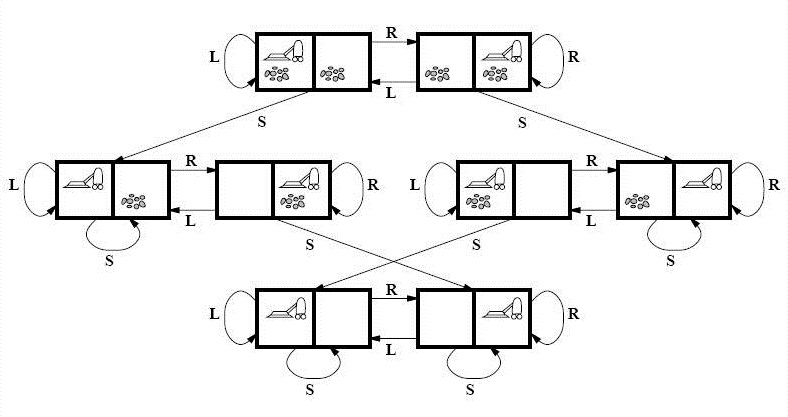
\includegraphics[scale=0.8]{./The-state-space-of-the-Vacuum-World-domain.jpg}
\end{center}



\end{document}